\documentclass{article}

  % if you need to pass options to natbib, use, e.g.:
  % \PassOptionsToPackage{numbers, compress}{natbib}
  % before loading nips_2018
  
  % ready for submission
  %\PassOptionsToPackage{numbers, compress}{natbib}
  \usepackage[final]{nips_2018}
  
  % to compile a preprint version, e.g., for submission to arXiv, add
  % add the [preprint] option:
  % \usepackage[preprint]{nips_2018}
  
  % to compile a camera-ready version, add the [final] option, e.g.:
  % \usepackage[final]{nips_2018}

  % to avoid loading the natbib package, add option nonatbib:
  % \usepackage[nonatbib]{nips_2018}
  
  \usepackage[utf8]{inputenc} % allow utf-8 input
  \usepackage[T1]{fontenc}    % use 8-bit T1 fonts
  \usepackage{hyperref}       % hyperlinks
  \usepackage{url}            % simple URL typesetting
  \usepackage{booktabs}       % professional-quality tables
  \usepackage{amsfonts}       % blackboard math symbols
  \usepackage{nicefrac}       % compact symbols for 1/2, etc.
  \usepackage{microtype}      % microtypography
  \usepackage{graphicx}
  \usepackage{multirow}
  %\usepackage{biblatex}
  %\addbibresource{proposal.bib}

  \title{Hate Speech Detection on Twitter}
  
  % The \author macro works with any number of authors. There are two
  % commands used to separate the names and addresses of multiple
  % authors: \And and \AND.
  %
  % Using \And between authors leaves it to LaTeX to determine where to
  % break the lines. Using \AND forces a line break at that point. So,
  % if LaTeX puts 3 of 4 authors names on the first line, and the last
  % on the second line, try using \AND instead of \And before the third
  % author name.
  
  \author{
    Jainul N.~Vaghasia\\
    Department of Computer Science\\
    University of Washington\\
    Seattle, WA 98105 \\
    \texttt{jnv3@cs.washington.edu}
    %% examples of more authors
    %% \And
    %% Coauthor \\
    %% Affiliation \\
    %% Address \\
    %% \texttt{email} \\
    %% \AND
    %% Coauthor \\
    %% Affiliation \\
    %% Address \\
    %% \texttt{email} \\
    %% \And
    %% Coauthor \\
    %% Affiliation \\
    %% Address \\
    %% \texttt{email} \\
    %% \And
    %% Coauthor \\
    %% Affiliation \\
    %% Address \\
    %% \texttt{email} \\
  }
  
  \begin{document}
  % \nipsfinalcopy is no longer used
  
  \maketitle

  \begin{abstract}
    We explore a neural network based method for classifying the presence of hate speech in a tweet.
    The network is based on word embeddings and mean pooling, and produces state-of-the art results on
    offline model. The method when combined with resampling of subset of past training data performs well
    under class imbalance in online setting. It is also speculated to be robust against concept drift in the stream.
  \end{abstract}
    
  \section{Introduction}
  Cyberbullying has become a rather common incident in that \citet{pew}
  found that, as of 2013, 73\% of people had witnessed harassment online, and a full
  40\% of people had experienced harassment directly. Such online harassment
  often includes posts with sexually violent language, threats, hate speech and degrading racist
  terms. Being able to identify cases of toxic tweets can therefore help in tackling this problem
  at its core. To that end, we frame a binary classification problem:
  given a tweet, we wish to determine whether a tweet is offensive or not. There is no
  agreed upon definition of ``offensive'' owing to the ambiguities in human communication, but we
  use the following specific definition provided by \citet{hateoffensive}: ``language that is used to express hatred towards
  a targeted group or is intended to be derogatory, to humiliate, or to insult the members of the group.''
  
  We then approach this problem with two different perspectives. First, we handle the tweets in
  an offline manner in which tweets are provided
  in a batch beforehand. Then we improve upon our model for online learning where
  tweets arrive at different time steps. In doing so, we address the class imbalance
  arising from the fact that offensive tweets are expected to be relatively fewer than non-offensive
  tweets (note the difference between witnessing an offensive tweet mentioned above and the presence
  of such tweet), and the concept drift that occurs when the distribution of such tweets changes
  based on socio-political events.

  All code was written on basic libraries and is available here: \url{https://github.com/JainulV/Hate-Detection-Twitter}

  \section{Datasets}
  In this paper, we deal with two datasets to train and evaluate our classifier. First dataset
  is \citet{hateoffensive}'s publicaly available HATE dataset compiled by searching for tweets on \url{www.Hatebase.org}.
  Tweets are binarized as ``hate speech'', or ``not''.
  The other dataset is \cite{Golbeck:2017:LLC:3091478.3091509}'s HAR harassment dataset, which identifies
  tweets as ``harassing'' or ``not''.\footnote{Available to researchers
  by emailing jgolbeck@umd.edu.} Retweets were removed from both datasets. Table~\ref{datasets-table}
  provides a numerical summary of both datasets.

  We also use 300 dimensional GloVe Common Crawl vector embeddings for translating words to vectors that are fed into our model
  (\citet{pennington2014glove}).

  \begin{table}
    \caption{Dataset Summary}
    \label{datasets-table}
    \centering
    \begin{tabular}{lll}
      \toprule
      %\multicolumn{2}{c}{Part}                   \\
      %\cmidrule(r){1-2}
      Name     & Labels and Counts     & Total \\
      \midrule
      \multirow{2}{*}{HATE} & Hate Speech \hspace{0.4cm} Not Hate Speech   &    \\
                             &  \hspace{0.2cm} \(1,430\) \hspace{2cm} \(23,353\) & $24,783$ \\
      \multirow{2}{*}{HAR} & Harassing \hspace{0.8cm} Not Harassing  &    \\
                             &  \hspace{0.2cm} $5,285$ \hspace{2cm} $15,075$ & $20,360$  \\
      \bottomrule
    \end{tabular}
  \end{table}

  \section{Methods}
  \subsection{Offline}
  Let us have \(\{(x^t, y^t)\}_{t=1}^n\) denote the training set where
  \(x^t\) is some tweet and \(y^t\) is the corresponding class label.
  We modify the TWEM method (\citet{kshirsagar2018predictive}) to use fewer parameters
  in exchange of minimal drop in accuracy. First, we create 300 dimenional embeddings for
  each word in a given tweet \(x^t\) of word length \(T\), so each word \(\{w_i\}_{i=1}^T\) in \(x^t\) is mapped to \(\{m_i\}_{i=1}^{T}\in \mathbb{R}^{300}\).
  Following this, we use mean pooling operation on \(\{m_i\}_{i=1}^T\), which allows us to capture the overall
  context of the tweet. Denote the output from this operation as \(a\). This representation \(a\) is then fed
  into a 50 node 2-layer MLP followed by ReLU activation to allow for nonlinear representation learning.
  This is the penultimate layer which passes to a fully connected softmax layer whose output is the probability
  distribution over the class labels.
  \subsection{Online}
  In order to adapt the above approach to online stream of tweets, we consider two queues of size \(L\)
  each, one holds the positive examples while the other holds the negative examples (\cite{Malialis2018QueueBasedRF}). Queue-based resampling stores the most recent example plus
  \(2L-1\) old ones. We will refer to the proposed algorithm as \(Queue_L\). The union of the two queues is then taken at each
  time step to form the new training set for the classifier. The cost function is given by
  \begin{equation} \label{eq:q}
      J=\frac{1}{|q^t|}\sum_{i=1}^{|q^t|} l(y_i, h(x_i)),
  \end{equation}
  where \(q^t\) is the union queue with \(|q^t|\leq 2L\) and \((x_i, y_i)\in q^t\). At each time step, the
  classifier is updated once according to \ref{eq:q}.

  The effectiveness of this approach can be attributed to the following highly intuitive reasoning. Having two queues keeps track of
  examples from both classes. It allows the classifier to ``remember'' old data from both classes, which can be seen as a form of oversampling to counteract the imbalance since the
  queue with less frequent examples will have same examples resampled more times than their counterparts. At the same time, we also note that since these queues are of
  fixed length \(L\), it allows the classifier to ``forget'' relatively old data and therefore act like a sliding window over the data stream. This forgetfulness is speculated to
  handle the concept drift present in the stream.

  \section{Experiments and Results}
  \subsection{Offline}
  To train the neural network, we perform minimal preprocessing which includes tokenizing the data using Spacy and applying GloVe Common Crawl vector embeddings. 
  Training is performed using gradient descent with \(\ell_2\) regularization to reduce overfitting. The regularization parameter
  was chosen to be \(0.001\) by cross validation on 80--20 training-validation split.
  
  For comparing our model on HATE dataset, we borrow features engineered by \cite{hateoffensive} (which include part-of-speech ngrams, sentiment analysis, and Twitter specific features) and apply logistic regression. In addition, we use the statistics for
  Naive Bayes baseline and GRU model that uses metadata like popularity, network reciprocity and subscribed lists provided by \cite{founta2018unified}.
  For HAR dataset,
  \cite{kshirsagar2018predictive} offer performance for a baseline model trained using logistic regression with character ngrams, word unigrams and TF*IDF.

  The results are compiled in Table \ref{offline-res}. It is evident that our model requires relatively fewer preprocessing steps and depends only on tweet text, which eliminates dependence on
  retrieving features like social graphs, sentiment readibility, etc. while performing better than these more complex approaches.

  \begin{table}
    \caption{Offline F1 Results}
    \label{offline-res}
    \centering
    \begin{tabular}{lll}
      \toprule
      %\multicolumn{2}{c}{Part}                   \\
      %\cmidrule(r){1-2}
      Method     & HATE     & HAR \\
      \midrule
      Logisitic Regression (\cite{kshirsagar2018predictive}) & - & 0.68\\
      Logisitic Regression (\cite{hateoffensive}) & 0.93 & -\\
      Naive Bayes & 0.82 & -\\
      GRU Text + Metadata (\cite{founta2018unified}) & 0.89 & -\\
      Ours & 0.94 & 0.70\\
      \bottomrule
    \end{tabular}
  \end{table}

  \subsection{Online}
  \begin{figure}
    \begin{center}
    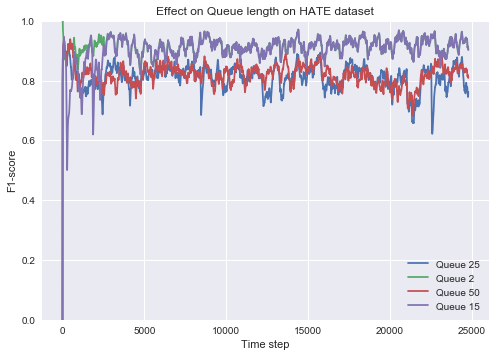
\includegraphics[width=3in]{Class_Imbalance_Result.png}
    \end{center}
    \caption{Prequential F1-Score against time step for different queue lengths}
    \label{fig:boat1}
  \end{figure}

  We begin by defining the prequential F1-score as our metric as suggested in \cite{Gama2012OnES}
  with a fading factor of \(\alpha=0.99\). At all time steps, we compute the prequential F1-score averaged over the most recent
  \(30\) runs.

  We inspect the performance of our algorithm \(Queue_L\) for \(L=\{2, 15, 25, 50\}\) as shown in Figure \ref{fig:boat1}. \(Queue_2\) is the quickest to learn and performs the best
  followed by \(Queue_{15}\) which eventually matches the performance
  of \(Queue_2\) at about 3000th time step. We speculate a trade-off here that deals with concept drift. It is also seen that
  \(Queue_{25}\) and \(Queue_{50}\) lead to excessive oversampling which forces the classifier to ``remember'' old data for a long time, thereby affecting
  the decision boundary. Consequently, they are not able to perform as good as the former algorithms.

  \section{Planned work}
  As seen above, we achieve state-of-the-art results on offline model and perform
  well on online model with imbalanced data. 
  Before the final paper submission, we expect to produce experimental evidence
  for the trade-off between concept drift and learning speed, or show that the given method fails under concept drift. 
  In addition, the online model is currently trained and evaluated only on the HATE dataset. Time permitting,
  we will also train and evaluate online model on the HAR dataset.

  \bibliographystyle{plainnat}
  \bibliography{milestone}

  \end{document}